\section{RRTPolar  Class Reference}
\label{classRRTPolar}\index{RRTPolar@{RRTPolar}}
Gradually bias the sampling towards the goal. 


{\tt \#include $<$rrt.h$>$}

Inheritance diagram for RRTPolar::\begin{figure}[H]
\begin{center}
\leavevmode
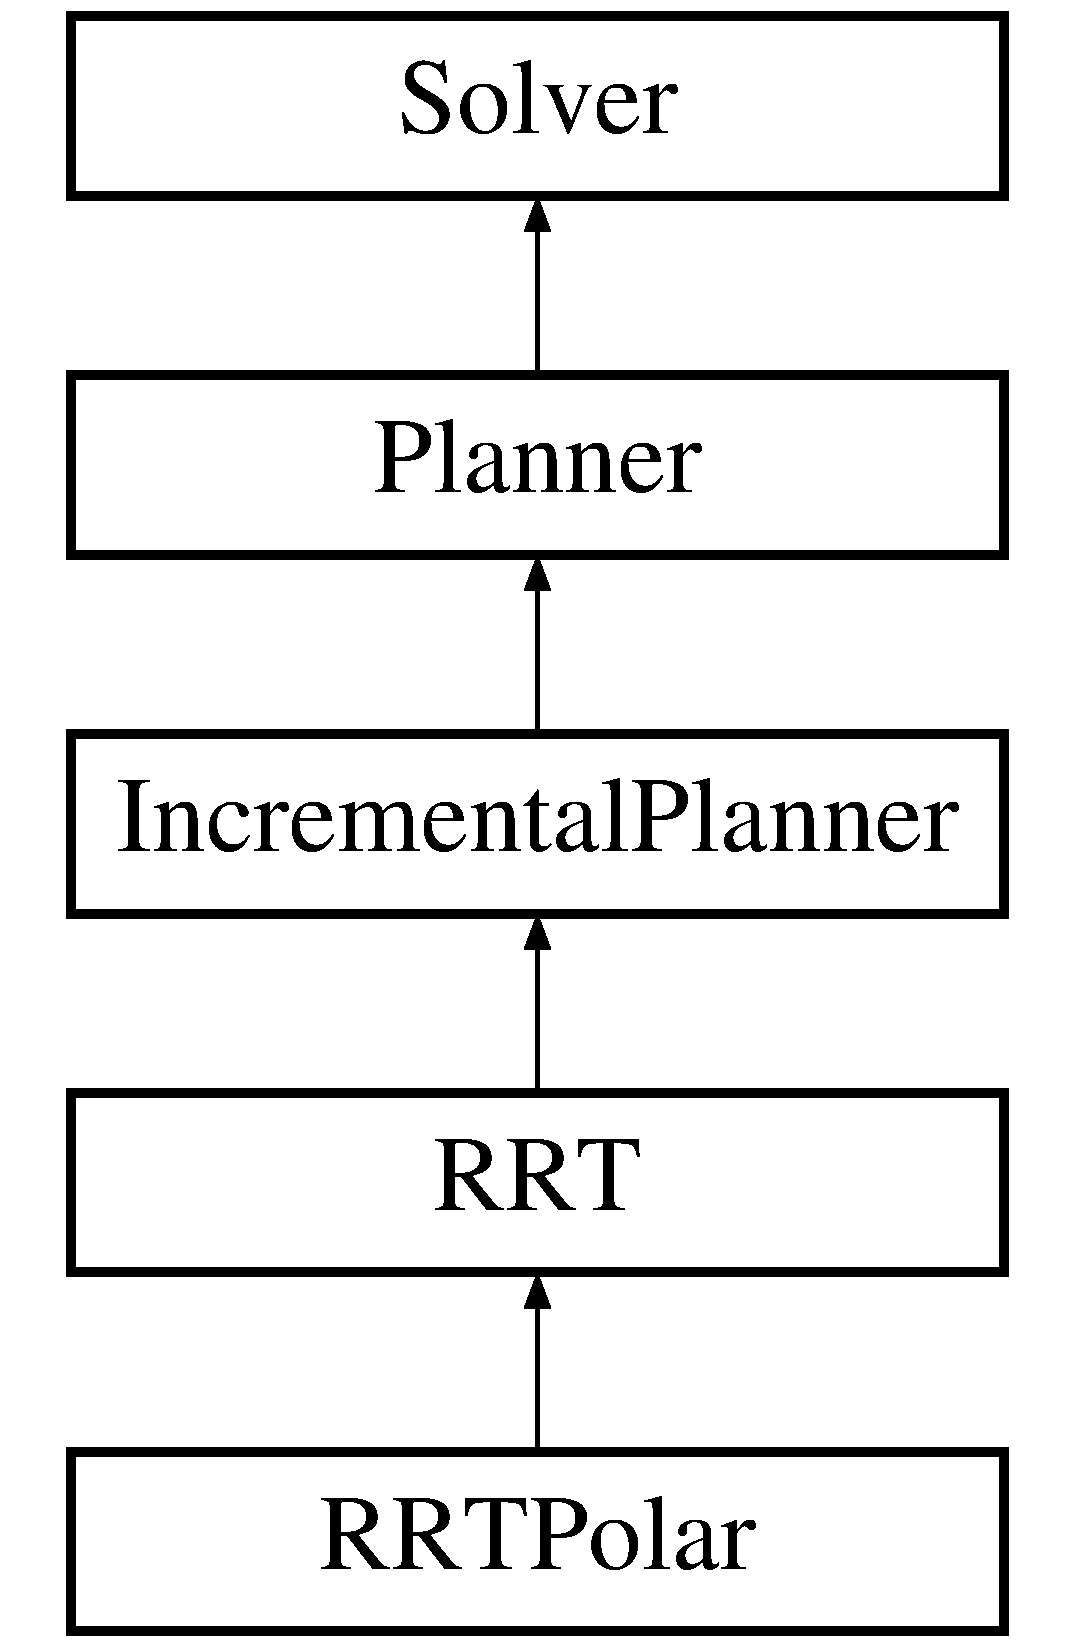
\includegraphics[height=5cm]{classRRTPolar}
\end{center}
\end{figure}
\subsection*{Public Methods}
\begin{CompactItemize}
\item 
{\bf RRTPolar} ({\bf Problem} $\ast$p)
\item 
virtual {\bf $\sim$RRTPolar} ()
\end{CompactItemize}
\subsection*{Public Attributes}
\begin{CompactItemize}
\item 
double {\bf Radius\-Exp}
\end{CompactItemize}
\subsection*{Protected Methods}
\begin{CompactItemize}
\item 
virtual {\bf MSLVector} {\bf Choose\-State} ()
\begin{CompactList}\small\item\em Pick a state using some sampling technique.\item\end{CompactList}\item 
virtual {\bf MSLVector} {\bf Select\-Input} (const {\bf MSLVector} \&x1, const {\bf MSLVector} \&x2, {\bf MSLVector} \&nx\_\-best, bool \&success)
\end{CompactItemize}


\subsection{Detailed Description}
Gradually bias the sampling towards the goal.

Instead of random sampling, this planner attempts to gradually bias  samples toward the goal. 



\subsection{Constructor \& Destructor Documentation}
\index{RRTPolar@{RRTPolar}!RRTPolar@{RRTPolar}}
\index{RRTPolar@{RRTPolar}!RRTPolar@{RRTPolar}}
\subsubsection{\setlength{\rightskip}{0pt plus 5cm}RRTPolar::RRTPolar ({\bf Problem} $\ast$ {\em p})}\label{classRRTPolar_a0}


\index{RRTPolar@{RRTPolar}!~RRTPolar@{$\sim$RRTPolar}}
\index{~RRTPolar@{$\sim$RRTPolar}!RRTPolar@{RRTPolar}}
\subsubsection{\setlength{\rightskip}{0pt plus 5cm}virtual RRTPolar::$\sim$RRTPolar ()\hspace{0.3cm}{\tt  [inline, virtual]}}\label{classRRTPolar_a1}




\subsection{Member Function Documentation}
\index{RRTPolar@{RRTPolar}!ChooseState@{ChooseState}}
\index{ChooseState@{ChooseState}!RRTPolar@{RRTPolar}}
\subsubsection{\setlength{\rightskip}{0pt plus 5cm}{\bf MSLVector} RRTPolar::Choose\-State ()\hspace{0.3cm}{\tt  [protected, virtual]}}\label{classRRTPolar_b0}


Pick a state using some sampling technique.



Reimplemented from {\bf RRT} {\rm (p.\,\pageref{classRRT_b4})}.\index{RRTPolar@{RRTPolar}!SelectInput@{SelectInput}}
\index{SelectInput@{SelectInput}!RRTPolar@{RRTPolar}}
\subsubsection{\setlength{\rightskip}{0pt plus 5cm}{\bf MSLVector} RRTPolar::Select\-Input (const {\bf MSLVector} \& {\em x1}, const {\bf MSLVector} \& {\em x2}, {\bf MSLVector} \& {\em nx\_\-best}, bool \& {\em success})\hspace{0.3cm}{\tt  [protected, virtual]}}\label{classRRTPolar_b1}




\subsection{Member Data Documentation}
\index{RRTPolar@{RRTPolar}!RadiusExp@{RadiusExp}}
\index{RadiusExp@{RadiusExp}!RRTPolar@{RRTPolar}}
\subsubsection{\setlength{\rightskip}{0pt plus 5cm}double RRTPolar::Radius\-Exp}\label{classRRTPolar_m0}




The documentation for this class was generated from the following files:\begin{CompactItemize}
\item 
{\bf rrt.h}\item 
{\bf rrt.C}\end{CompactItemize}
